% $Id: Note1.tex,v 1.1 2022/11/15 22:36:13 pjanzen Exp $
\documentclass[10pt]{article}
\usepackage{graphicx}
\textwidth=7.25in
\textheight=9.6in
\oddsidemargin=-.35in
\topmargin=-.80in
%\footskip=1in
\setcounter{secnumdepth}{2}
%\pagestyle{empty}
\begin{document}

\begin{center}
{\large{\sc Quirks in xmap}}
\end{center}

Histogram data from the spacecraft is binned in pixels of 6-degree
latitude, with one pixel centred at the NEP (or, more accurately,
closest-to-NEP).

\texttt{xmap} by default, and the ISOC, show pixels of 6 degree latitude,
with the pixel \emph{edge} at NEP.

What this means is that rounding shifts the ribbon from where it ought to
be, in the default maps shown.  The ribbon appears where it ought to be in
most other maps, like Abrate and HEALpix.

The ISOC's 6-by-7-degree smearing mitigates the effect for them, and
turning on this effect in \texttt{xmap} mitigates the effect for us.

% Don't forget 'R' to make things sensible!

Demonstration of issue:
\begin{quotation}
\vspace{-5mm}
\noindent \begin{verbatim}
% xmap 11 500
\end{verbatim}
Input:
\begin{quotation}
\noindent \begin{verbatim}
	sb 60 90 0 90
	t 11 500
	sb 60 30 0 90
	sF 1
	sf /home/pjanzen/id/1-deg/qABC/ .qABC
	t 11 500
	t 11 500
	sb 60 90 0 90
\end{verbatim}
\end{quotation}
\end{quotation}

This results in 4 maps.

Map 1 is histogram 6-degree data, mapped into pixels of 2 degrees latitude
by six degrees longitude.  It has a lot of black bars, because all the
six-degree data is being put into one 2-degree strip with empty bins
surrounding in latitude.

Map 2 is like map 1, but with the traditional 6x6 pixels.  This is the
default \texttt{xmap} product.

If you switch between maps 1 and 2, they look like the same underlying
data.

Maps 3 and 4 are the same thing respectively as maps 2 and 1, only
constructed out of 1-degree data files made from the direct events.
There aren't gaps in map 4 like there are in map 1, because 1-degree data
fits fine into 2-degree bins.  Map 4 just looks a little noisy.  Of course,
again, maps 3 and 4 look like the same underlying data.

Map 4 and Map 1 also look like representations of the same underlying data
-- it's just that map 1 has black bars.

But maps 2 and 3 -- the two 6-degree-latitude maps, one made from 6-degree
data and one made from 1-degree data -- do \emph{not} look the same.

If one does HEALpix or Abrate, even out of the 6-degree data, it matches
all but map 2.  For example:

\begin{quotation}
\vspace{-5mm}
\noindent \begin{verbatim}
% xmap 11 500
\end{verbatim}
\begin{quotation}
\noindent \begin{verbatim}
	t 11 500
	sh 15
	t 11 500
	sa 1800
\end{verbatim}
\end{quotation}
\end{quotation}

\noindent are what made Maps 5 and 6.

To obtain the pixel index for a given latitude and longitude,
\texttt{mappage.c:get\_pixel\_value()} gets called.  It spins off to
\texttt{healpix\_ndx()} or \texttt{abrate\_ndx()} if needed, but otherwise
does integer truncation:
\begin{quotation}
\vspace{-5mm}
\noindent \begin{verbatim}
		i = (180. + lng) / 360. * pltnlng;
		j = (90. - lat) / 180. * pltnlat;
		return(pltdata[j * pltnlng + i]);
\end{verbatim}
\end{quotation}


\newpage
\begin{figure}
\begin{center}
\noindent
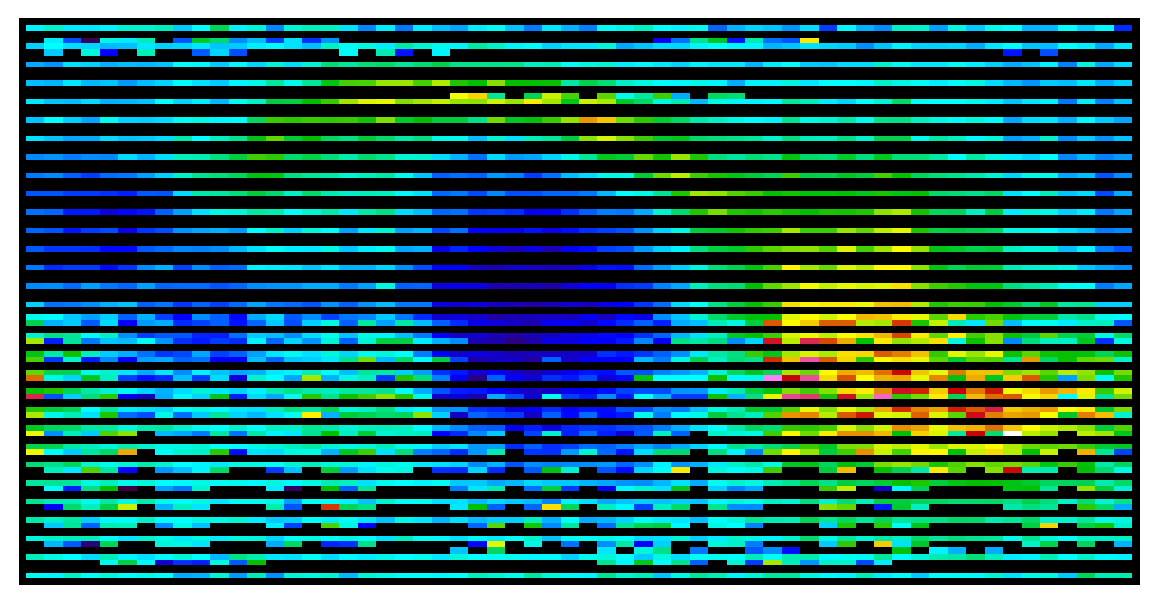
\includegraphics[width=0.45\textwidth]{map1}
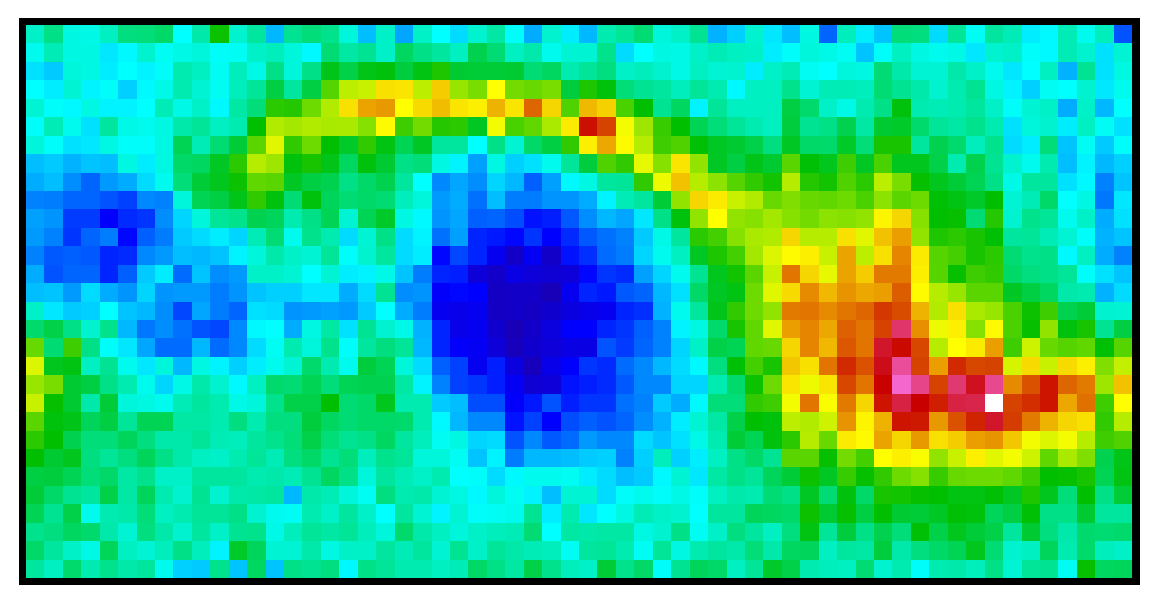
\includegraphics[width=0.45\textwidth]{map2}

\noindent
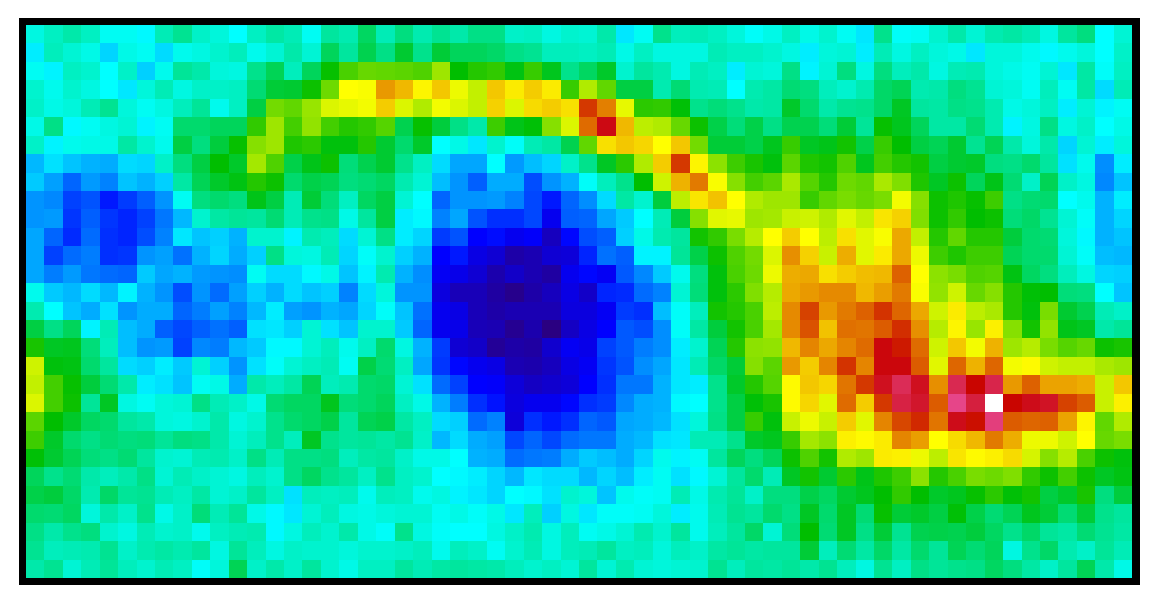
\includegraphics[width=0.45\textwidth]{map3}
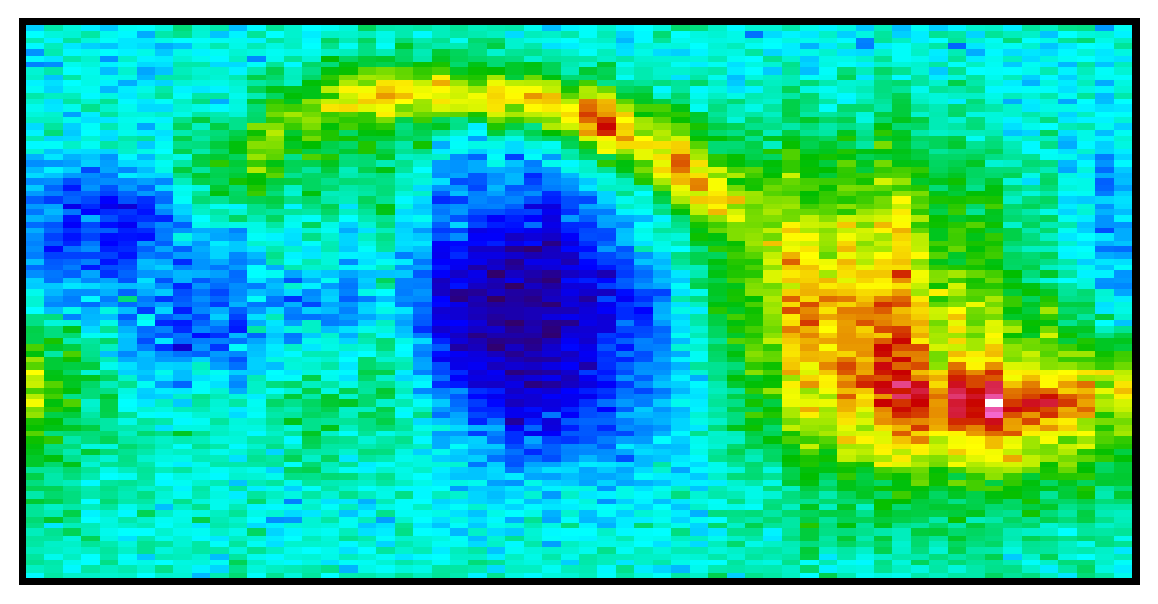
\includegraphics[width=0.45\textwidth]{map4}

\noindent
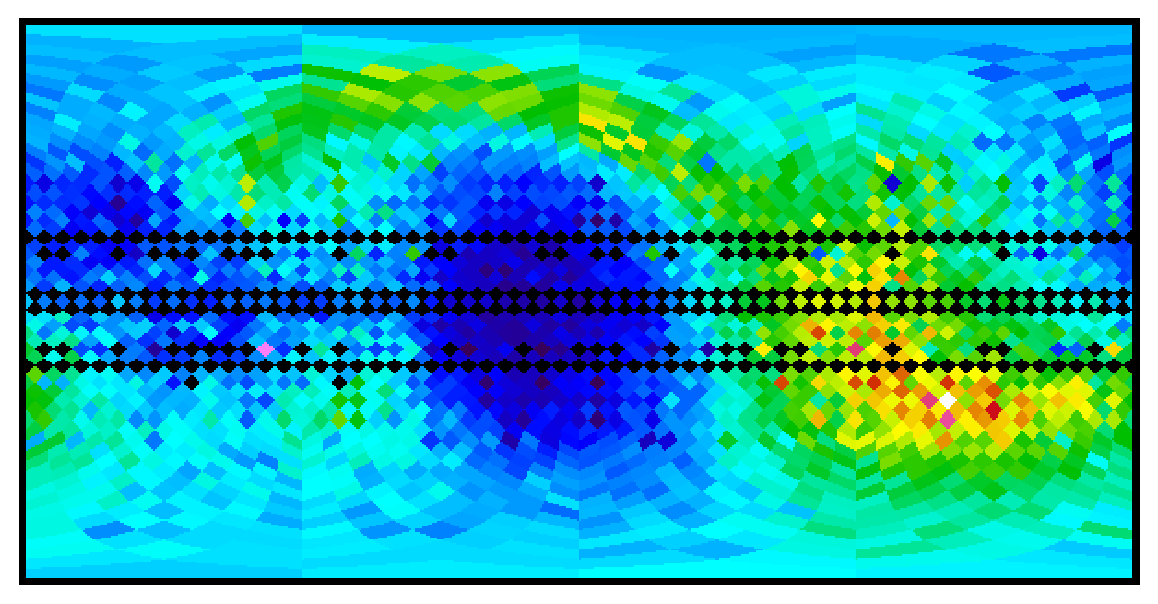
\includegraphics[width=0.45\textwidth]{map5}
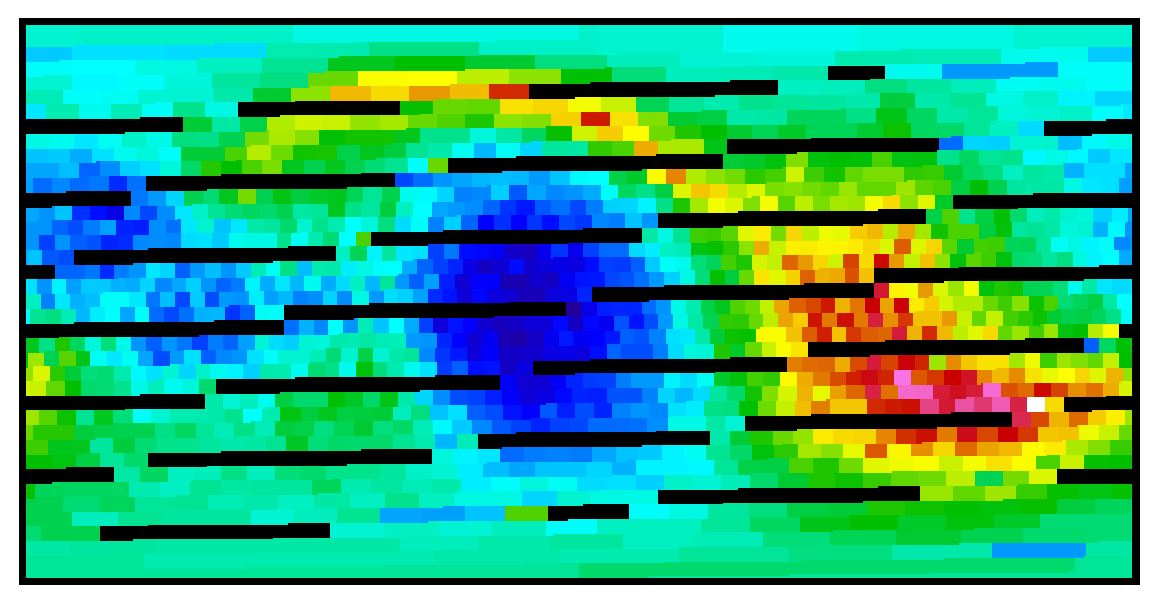
\includegraphics[width=0.45\textwidth]{map6}
\end{center}

\caption{IBEX-Hi data summed over orbits 11-500.\\
First map: $6^\circ \times 2^\circ$ longitude/latitude map made of
histogram data.\\
Second map: $6^\circ \times 6^\circ$ longitude/latitude map made of
histogram data.\\
Third map: $6^\circ \times 6^\circ$ longitude/latitude map made of
direct event data binned at $1^\circ$ along the spin axis.\\
Fourth map: $6^\circ \times 2^\circ$ longitude/latitude map made of
direct event data binned at $1^\circ$ along the spin axis.\\
Fifth map:  HEALpix version of histogram data.\\
Sixth map:  Abrate version of histogram data.\\
The point is that the ribbon appears to be in a different location in map
2, due to rounding/shifting between the histogram binning and the map
binning, which are essentially $3^\circ$ offset in latitude.}
\end{figure}
\end{document}
